\chapter{Background}

\section{Large Language Models and the Transformer Architecture}

Modern large language models (LLMs) are built on the Transformer architecture, which introduced the self-attention mechanism as a replacement for recurrent or convolutional networks in sequence modeling. In the seminal “Attention is All You Need” paper \cite{vaswani2023attentionneed}, the authors showed that a Transformer using only attention could achieve state-of-the-art results in machine translation, with faster training and better parallelism. The attention mechanism allows a model to weigh the relevance of different words in the input when producing each part of the output, effectively letting the model “focus” on important context. Multiple attention “heads” capture different relationships in parallel, enabling rich representations of language. This architecture is the backbone of today’s LLMs and is largely responsible for their ability to capture long-range dependencies and complex patterns in text.
\newline

\begin{figure}[h]
\centering
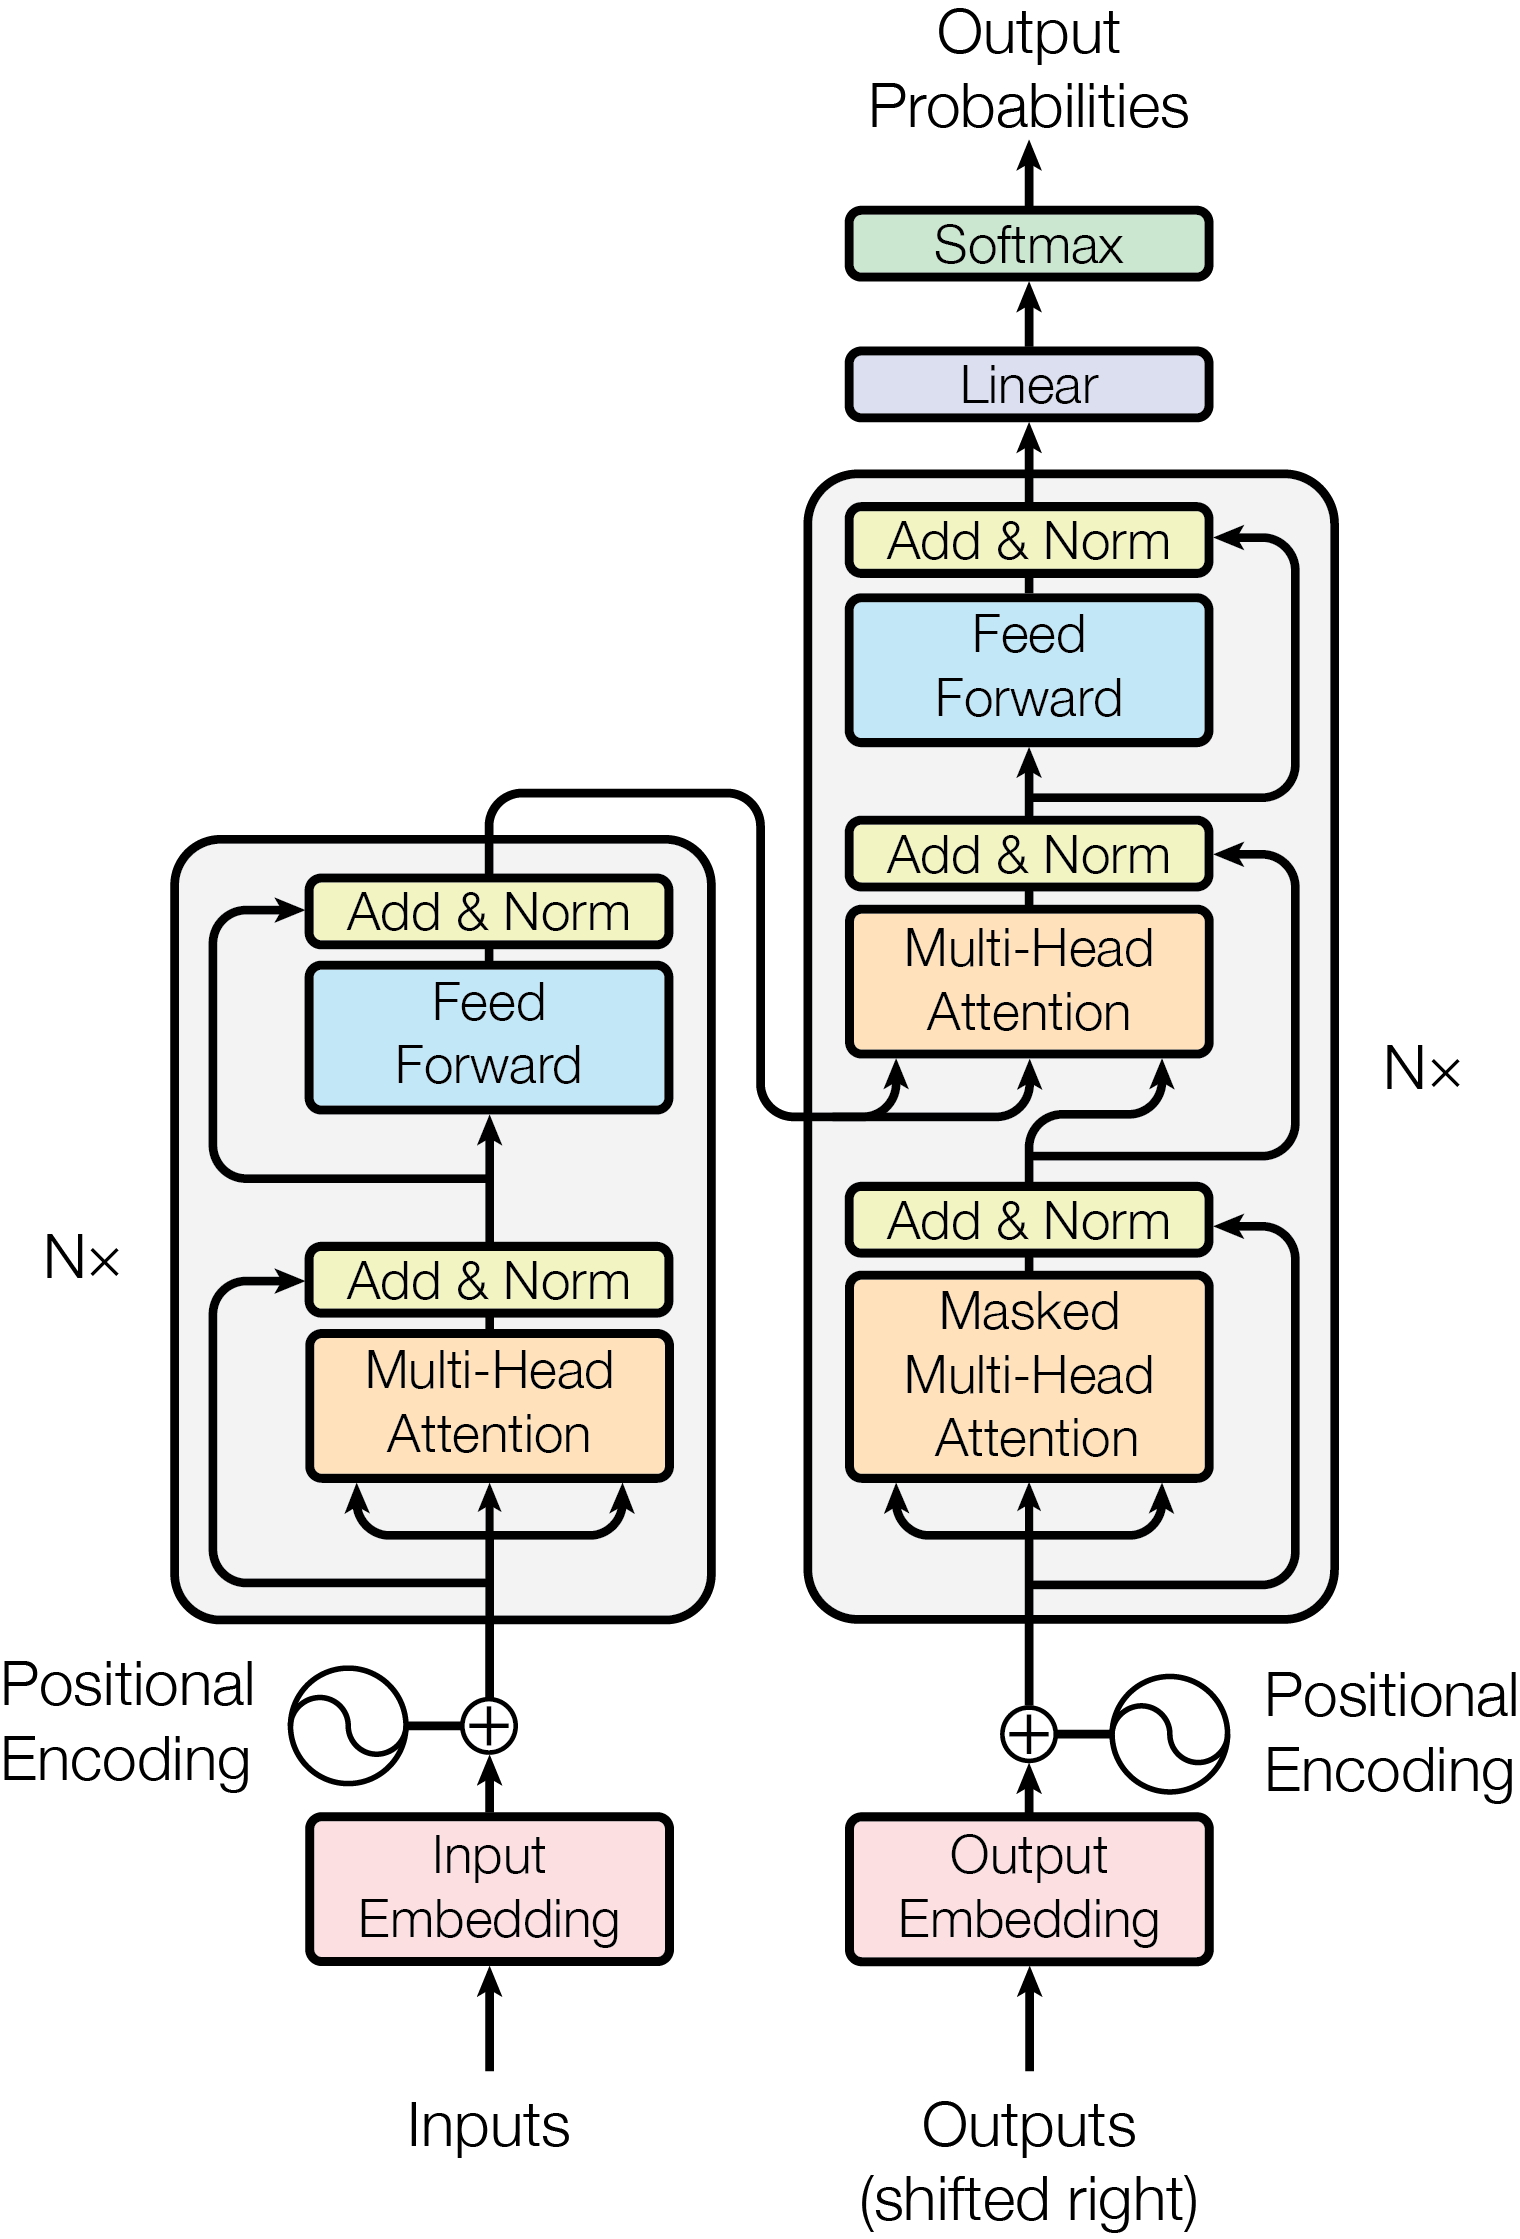
\includegraphics[width=0.35\textwidth]{figures/transformer.png}
\caption{The Transformer - model architecture \cite{vaswani2023attentionneed}}
\end{figure}

Crucially, LLMs are trained on massive corpora of text via self-supervised learning (predicting the next word or masked words). This scaling of model size and data has led to emergent capabilities. Notably, GPT-3 (175 billion parameters) demonstrated that simply making models larger unlocks in-context learning abilities: GPT-3 could perform many tasks without gradient updates or fine-tuning, given only a prompt with a few examples or an instruction. In their paper “Language Models are Few-Shot Learners” \cite{brown2020languagemodelsfewshotlearners}, Brown et al. showed that GPT-3, when prompted with a task description and a few input-output examples (known as few-shot), achieved strong results on translation, question-answering, and other NLP tasks. The same model can solve diverse tasks zero-shot or few-shot by understanding the task from its prompt. Performance on many benchmarks approached that of models explicitly fine-tuned on those tasks. This revealed that very large transformers inherently learn to follow instructions and examples given in the prompt, essentially “programming” the model through natural language.
\newline

\begin{figure}[h]
\centering
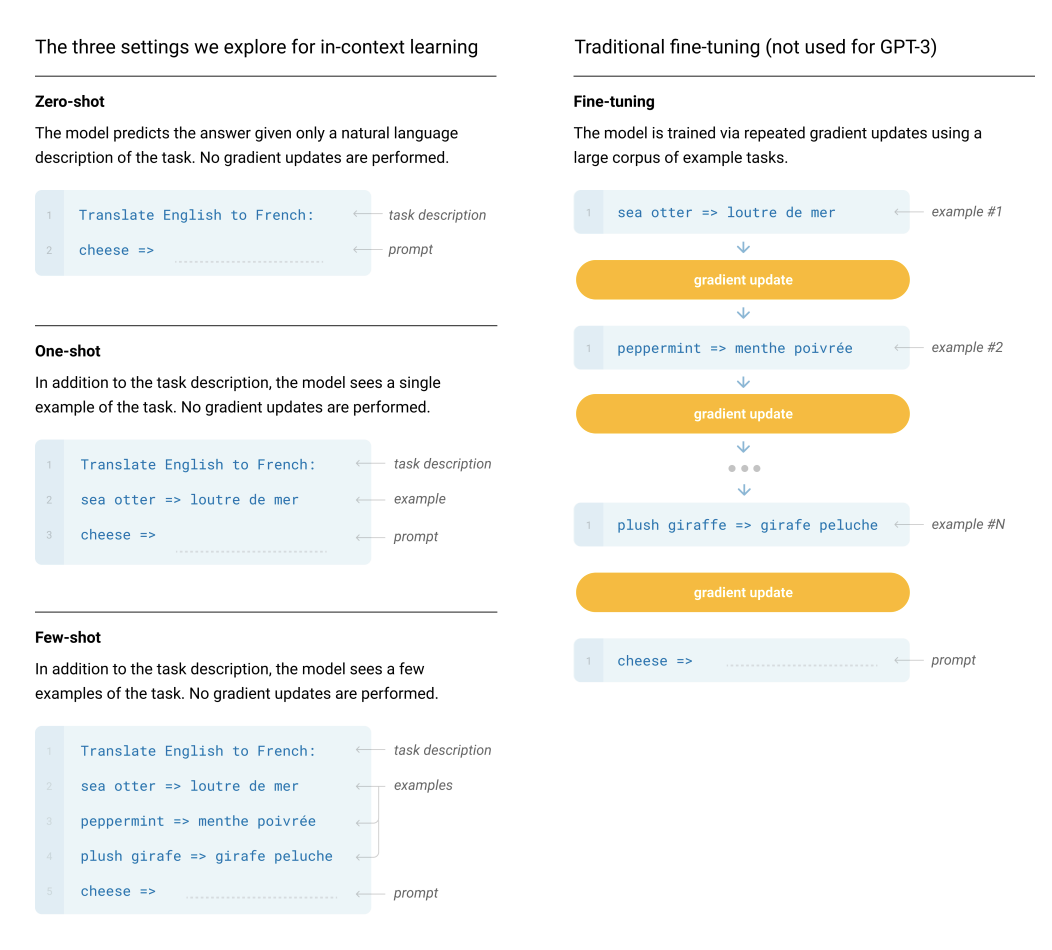
\includegraphics[width=0.85\textwidth]{figures/few_shot_example.png}
\caption{Zero-shot, one-shot and few-shot, contrasted with traditional fine-tuning \cite{brown2020languagemodelsfewshotlearners}}
\label{few-shot}
\end{figure}

At the same time, the authors noted limitations, some tasks still stumped the model and it sometimes produced incorrect or nonsensical outputs (due to data biases or reasoning limits). These failure modes foreshadow issues like hallucination that we discuss later. Nonetheless, the Transformer based LLM paradigm of pretraining on broad data, then prompting the model for downstream tasks, has become the foundation for current AI systems.

\section{Prompting Techniques for LLMs}

Because LLMs can understand and follow prompts, a new field of “prompt engineering” has emerged to get the best performance from them. A variety of prompting techniques have been developed to improve accuracy, reasoning, and reliability.
\newline

In zero-shot prompting, we just give the model an instruction or question and ask for an answer. Large models like GPT-3 were surprisingly capable in the zero-shot setting \cite{brown2020languagemodelsfewshotlearners}, but performance often improves if we provide more guidance.
\newline

In few-shot prompting (in-context learning) as shown in figure \ref{few-shot}, the prompt includes a handful of examples of the task with inputs and desired outputs, before the actual query. This “demonstration” primes the model on the task format and desired behavior. The GPT-3 work showed that with enough parameters, models can rapidly generalise from just a few examples provided in the prompt \cite{brown2020languagemodelsfewshotlearners}. For instance, given two or three example translations (English–French), GPT-3 can translate a new sentence without any fine-tuning. Few-shot prompts essentially perform on-the-fly conditioning of the model, and the order and choice of examples can affect performance. Researchers found that prompt design details (e.g. example ordering) can be important, a phenomenon dubbed prompt order sensitivity \cite{lu2022fantasticallyorderedpromptsthem}. Best practices (such as “fantastically ordered prompts” have been proposed to choose and order demonstrations to maximise accuracy.
\newline

In instruction prompting, rather than examples, we can give a clear natural language instruction. Instruction-tuned models (like InstructGPT \cite{ouyang2022traininglanguagemodelsfollow} or ChatGPT) have been further trained to better follow explicit instructions. For instance, a prompt like: “Summarise the following text in one paragraph.” will guide the model’s behavior. The success of instruction tuning shows that models can internalise a general notion of following user commands.
\newline

In chain-of-thought (CoT) prompting, one major advance for reasoning tasks is to prompt the model to produce a step-by-step reasoning trace before giving the final answer \cite{wei2023chainofthoughtpromptingelicitsreasoning}. In chain-of-thought prompting, we include in the prompt an example of a question followed by a human-like reasoning process (a series of steps or thoughts) concluding with the answer. When the model is prompted to “Let’s think step by step,” it will output a chain of logical steps and then an answer. Wei et al. \cite{wei2023chainofthoughtpromptingelicitsreasoning} showed this dramatically improves performance on arithmetic word problems, commonsense reasoning, and other tasks that require multi-step thinking. The improvement is so substantial that chain-of-thought was identified as an emergent ability of sufficiently large models, smaller models cannot do it well, but models with tens of billions of parameters suddenly can. For example, a 540B model given 8 examples of chain-of-thought reasoning achieved state-of-the-art on the GSM8K \cite{cobbe2021trainingverifierssolvemath} math word problem benchmark, outperforming even some fine-tuned approaches \cite{wei2023chainofthoughtpromptingelicitsreasoning}. The model effectively “reasons out loud,” reducing errors in tasks like math where keeping track of partial results is crucial.
\newline

\begin{figure}[h]
\centering
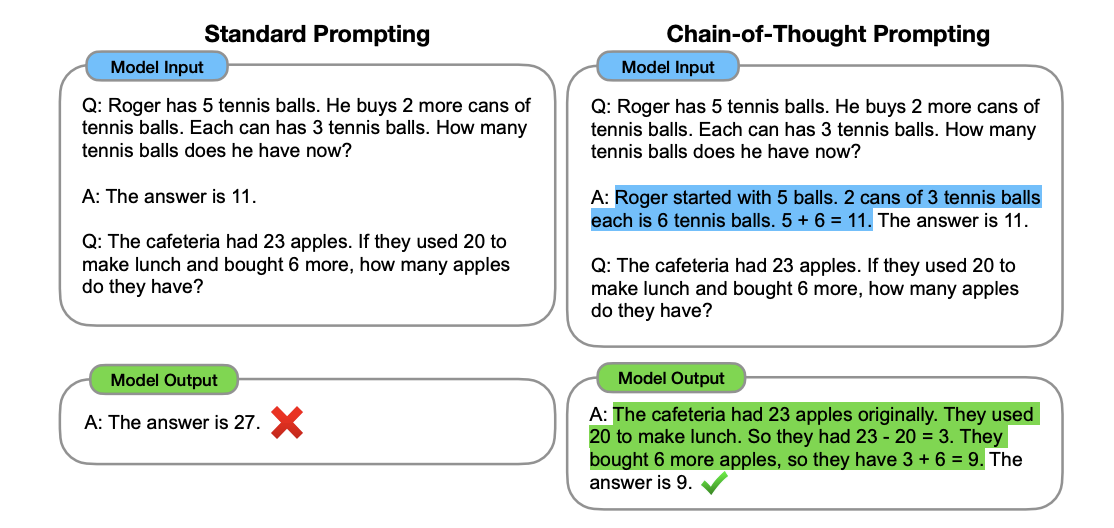
\includegraphics[width=0.85\textwidth]{figures/chain-of-thought.png}
\caption{Chain of thought prompting \cite{wei2023chainofthoughtpromptingelicitsreasoning}}
\end{figure}

An intriguing variant is Zero-Shot CoT, proposed by Kojima et al. \cite{kojima2023largelanguagemodelszeroshot}, simply appending a phrase like “Let’s think step by step.” to the prompt often triggers the model to produce a chain of reasoning, even without any examples. This trick enabled strong performance on reasoning benchmarks, for instance, accuracy on a math dataset (MultiArith \cite{roy2016solvinggeneralarithmeticword}) jumped from 17.7\% to 78.7\% by adding that prompt phrase for an InstructGPT model \cite{kojima2023largelanguagemodelszeroshot}. This demonstrates that models have latent reasoning abilities that the right prompt can unlock.
\newline

In self-consistency decoding, after obtaining a chain-of-thought, one can further boost reliability by using self-consistency. Instead of taking the model’s first answer, we sample the model multiple times (each time it may produce a different reasoning chain and answer). We then aggregate the answers (e.g. by majority vote). Wang et al. \cite{wang2023selfconsistencyimproveschainthought} found that this method significantly improved accuracy on reasoning tasks, the most consistent answer across multiple sampled reasoning paths is usually correct. For example, with GSM8K math problems, self-consistency improved accuracy by nearly 18\% versus a single chain-of-thought \cite{wang2023selfconsistencyimproveschainthought}. The intuition is that complex problems often have multiple ways to reach the solution, and if many independent reasoning attempts converge on the same answer, it’s likely correct. Self-consistency also reduces sensitivity to any one flawed chain-of-thought or particular phrasing of the prompt.
\newline

Scratchpad prompting \cite{nye2021workscratchpadsintermediatecomputation} is similar to CoT, encouraging the model to work out intermediate calculations explicitly. We also have prompts that induce the model to verify or reflect on its answer (e.g. generate a solution, then generate a “check” or critique). These approaches aim to reduce mistakes by leveraging the model’s own capabilities in a multi step prompt. As an example, prompting a model to “reflect on whether the answer could be wrong and why” can catch obvious errors and have it correct itself in a second attempt.
\newline

Overall, these techniques show that how you prompt an LLM can be as important as what task you ask, the prompt shapes the model’s behavior profoundly. As a result, prompt design has evolved from simple Q\&A examples to sophisticated strategies that elicit reasoning and self checking. These methods drive the idea that the prompt itself can teach or guide the model without changing the model’s weights. This forms the basis for building more complex LLM-driven systems.

\section{LLM Agents and Pipeline Architectures}

While a well-crafted single prompt can often get impressive results, there are limits to what an LLM can do in one go, especially for complex, knowledge-intensive, or interactive tasks. This has motivated the development of LLM based agents and multi-step pipeline architectures that go beyond a single prompt and response. These architectures integrate the LLM with additional tools or break problems into smaller sub-tasks, often yielding greater accuracy and flexibility. We discuss two prominent architectures: ReAct \cite{yao2023reactsynergizingreasoningacting} and Retrieval Augmented Generation \cite{yang2018hotpotqadatasetdiverseexplainable}, as examples of LLM agents and retrieval-based pipelines, respectively.
\newline

\subsection{ReAct}

ReAct (Reasoning + Acting) is a framework that combines the strengths of chain-of-thought reasoning with the ability to take actions (such as calling external tools or querying a database) in an interleaved manner. In a ReAct agent, the LLM’s output is structured to alternate between reasoning traces (thinking steps in natural language) and action commands that the agent executes in an environment or via an API. For example, faced with a question, the model might reason “I should look up this person’s birthdate” (reasoning) and then output an action like \texttt{SEARCH("Person Name birthdate")}. The agent executes the search, retrieves results, and feeds them back to the model, which continues reasoning with the new information, and so on. By explicitly prompting the model to both “think” and “act,” ReAct creates a closed loop where the model can gather evidence and update its plan. This combination of reasoning and acting enables more powerful problem-solving.
\newline

Critically, the reasoning trace helps the model decide which action to take next and how to handle the tool outputs, while the tools ground the model’s knowledge and reduce hallucinations. Yao et al. demonstrated ReAct on tasks like factual question answering (with a Wikipedia search API) and interactive decision-making (in a text-based game environment) \cite{yao2023reactsynergizingreasoningacting}. On knowledge tasks such as HotpotQA \cite{yang2018hotpotqadatasetdiverseexplainable} (multi-hop QA) and FEVER \cite{thorne2018feverlargescaledatasetfact} (fact verification), ReAct was able to reduce hallucination and error propagation by retrieving relevant facts before final answer generation \cite{yao2023reactsynergizingreasoningacting}. The model’s chain-of-thought ensures that it uses the retrieved information effectively and provides a rationale, resulting in more interpretable and trustworthy outputs compared to a black-box prompt that directly answers. For instance, rather than guessing an answer from its parametric memory (and possibly getting it wrong), a ReAct agent will explicitly say “According to the article I found, the person was born in 1980”, tying the answer to an external source.
\newline

In interactive environments (like an ALFWorld household task \cite{shridhar2021alfworldaligningtextembodied} or the WebShop online shopping task \cite{yao2023webshopscalablerealworldweb}), ReAct significantly outperformed traditional reinforcement learning agents, despite using only a few in-context examples for prompting \cite{yao2023reactsynergizingreasoningacting}. The ability to maintain a high-level plan in the reasoning while executing step-by-step actions is key. Overall, ReAct exemplifies why one would build a more complex LLM-based agent: a plain prompt might hallucinate missing facts or be unable to interact with external systems, whereas an agent can dynamically query tools, navigate environments, and correct itself using intermediate results.

\begin{figure}[h]
\centering
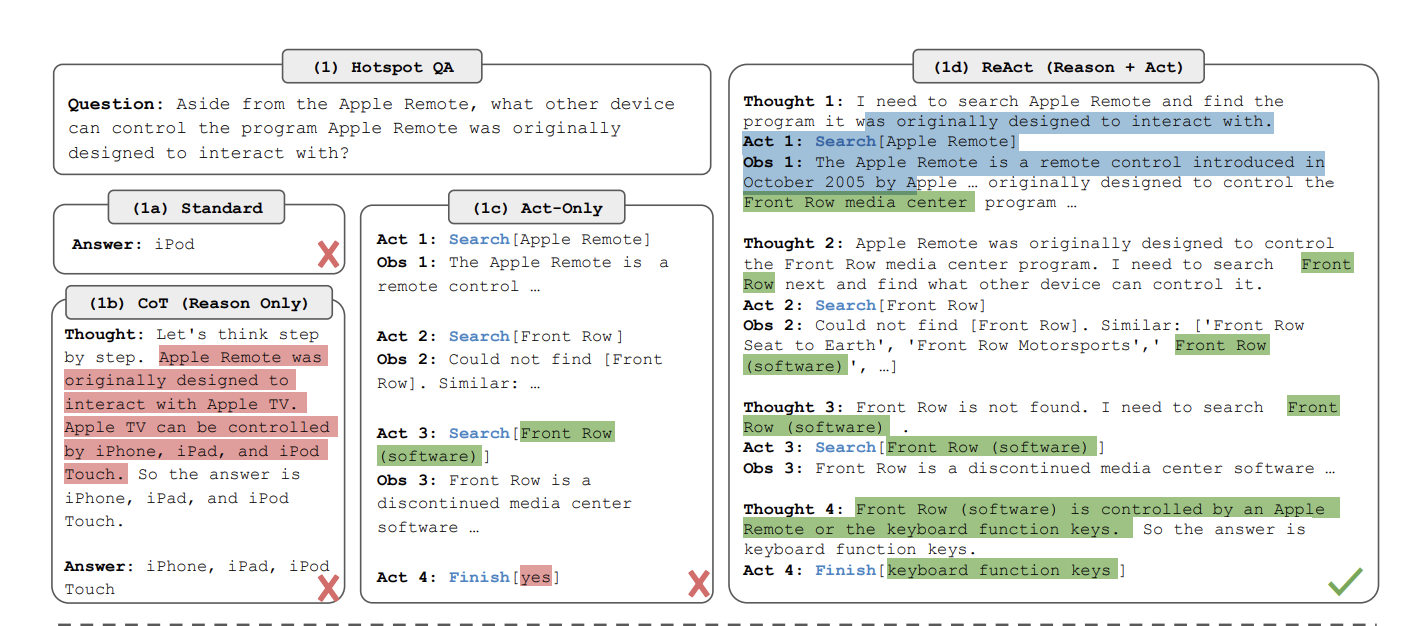
\includegraphics[width=0.95\textwidth]{figures/react.png}
\caption{(1) Comparison of 4 prompting methods, (a) Standard, (b) Chain-of-thought (CoT, Reason Only), (c) Act-only, and (d) ReAct (Reason+Act), solving a HotpotQA  question. \cite{yao2023reactsynergizingreasoningacting}}
\end{figure}

\subsection{Retrieval-Augmented Generation}

Retrieval-Augmented Generation (RAG) \cite{lewis2021retrievalaugmentedgenerationknowledgeintensivenlp} is another powerful architecture that combines an LLM with a dedicated retrieval system, forming a pipeline that first fetches relevant context from a knowledge source and then generates the answer. In the original RAG framework, a large Transformer-based generative model is augmented with a non-parametric memory (e.g. a vector-indexed Wikipedia) that it can query. When asked a question, the system uses a retriever to pull, say, the top-$k$ text passages related to the query. Those passages are then provided to the LLM as additional context in the prompt, and the model is tasked with producing an answer that integrates that information.
\newline

The key benefit is that the LLM is no longer limited to the facts stored in its fixed weights, it has an external knowledge base it can utilise. Lewis et al. showed that a RAG model fine-tuned on open-domain QA achieved state-of-the-art results on several benchmarks, outperforming models that relied only on parametric memory \cite{lewis2021retrievalaugmentedgenerationknowledgeintensivenlp}. Moreover, the outputs were judged to be more specific and factually accurate than those from a comparable model without retrieval. By design, RAG provides a traceable origin of information since the model’s answer can be linked to the retrieved sources, which is important for trust and verification. RAG based pipelines have become popular in industry for building domain-specific assistants: e.g., a legal assistant LLM can be connected to an internal document repository so that it always cites the relevant policy or law rather than hallucinating. The retrieval component can be updated independently (e.g. add new documents) without retraining the language model, making maintenance easier. Beyond QA, retrieval is used in tasks like long-form summarisation (retrieve related references), dialogue (recall facts mentioned earlier or user profile info), etc. Essentially, whenever current knowledge or reference to source material is needed, a RAG architecture is beneficial. It’s an example of a more complex pipeline that solves a problem a raw LLM cannot. No matter how big the model, it might not know about events from after its training cutoff, but a retrieval module can fetch up-to-date info for it to use.
\newline

Both ReAct and RAG illustrate why developers compose LLMs into larger tool-using pipelines or agents. A plain LLM prompt is a single-shot attempt at the task, which may fall short if the task requires multiple steps of reasoning, external knowledge, or interacting with an environment. By adding structure around the LLM, we can overcome these limitations. An LLM agent can decompose a task (explicitly thinking step by step, using sub-results) and invoke external tools (e.g. search engines, calculators, databases, APIs) to handle subtasks that the LLM isn’t reliable at. This often yields better results than a monolithic prompt. For example, even an LLM can make arithmetic mistakes on large numbers if prompted directly, but an agent that calls a calculator will get it exactly right. Similarly, rather than expecting the LLM to internally know every fact (which leads to hallucination when it doesn’t), a RAG pipeline compels it to base answers on retrieved documents. There is also a modularity benefit: one can upgrade the retriever or add new tools without changing the core LLM.
\newline

This added complexity, however, comes with new challenges, especially in ensuring these multi-step systems are reliable. We next examine common failure modes that can occur in LLM agents and pipelines.

\section{Common Failure Modes of LLMs and Agents}

Despite their impressive capabilities, LLMs are far from infallible. They exhibit several failure modes - tendencies to produce incorrect or undesired outputs, which can be exacerbated in complex agent or pipeline settings. Understanding these failure modes helps motivate techniques (like prompt optimisation and human feedback) to mitigate them.
\newline

One well-known issue is hallucination. An LLM is said to hallucinate when it fabricates information that is not grounded in reality or provided sources. For example, an LLM might confidently state a wrong date or cite a non-existent article. Hallucinations often arise in open-ended generation when the model’s training data lead it to produce a reasonable sounding answer that is false. This is especially problematic in factual tasks. With a standard prompt, the model might not admit ignorance and instead “guess” an answer.
\newline

In multi-step agents, hallucination can manifest as the agent hallucinating intermediate steps or tool outputs that haven’t actually been verified. For instance, a ReAct agent might generate a reasoning step saying “(Search result shows X)”, when in fact no such result was found, effectively hallucinating the content of a tool’s output. The ReAct paper \cite{yao2023reactsynergizingreasoningacting} explicitly noted that a pure chain-of-thought approach without tool use was prone to error propagation. The model might assume a false fact in its reasoning and then stick with it to the final answer. By introducing real tool results, ReAct aimed to break that cycle. However, if the agent’s prompt isn’t carefully designed, it might ignore the tool output or misuse it, still leading to incorrect answers. Retrieval-augmented generation systems also face a related failure mode, if the retriever pulls irrelevant passages or if the model doesn’t properly incorporate the evidence, the final answer can be wrong or only loosely related to the query. In other words, having a tool or context doesn’t guarantee it’s used correctly. Thus the prompts guiding the agent must enforce faithfulness (e.g. “use the retrieved document to justify your answer”). If the prompt is weak, the model might revert to its parametric knowledge and hallucinate an answer that conflicts with the retrieved data.
\newline

Another failure mode is inability to follow instructions or format when the prompt is suboptimal. LLMs can be very sensitive to prompt phrasing. A slight ambiguity or a missing detail in instructions can lead the model astray. For example, if an agent’s prompt doesn’t explicitly tell the model when to stop reasoning, the model might go into an endless loop of tool calls. Or if the prompt for a multi-step task is under-specified, the model might skip necessary steps. It has also been observed that even changing the order of few-shot examples or wording of a single instruction can substantially alter performance \cite{lu2022fantasticallyorderedpromptsthem}. As a result, pipelines and agents often require extensive manual prompt trial-and-error to become reliable. This brittleness is a key motivator for prompt optimisation methods later discussed.
\newline

In complex multi-turn interactions, context handling can fail. A chatbot agent might forget important details given earlier (context window limits) or confuse information from different turns. An agent might also inadvertently reveal private tool outputs or system instructions if the prompt is not well constructed to prevent that (a kind of prompt leakage), and in production systems these risks can be exploited via prompt injection \cite{liu2024automaticuniversalpromptinjection,reddy2025echoleakrealworldzeroclickprompt,zheng2023judgingllmasajudgemtbenchchatbot}. Once again these failure modes trace back to prompt content and how the agent is directed to manage memory and confidentiality.
\newline

It’s worth noting that evaluating some of these failures itself is non-trivial. Determining whether an LLM’s answer is correct can be as hard as the answering the original question. If the question requires expert knowledge, an automated system may not easily verify the answer’s correctness without that same knowledge. This is why many LLM answers need human review, and why automatic evaluation often struggles (we delve into evaluation frameworks next). An implication is that building a reliable agent often becomes an iterative process, identify a failure (model gave a wrong or nonsensical result), then adjust the prompt or pipeline to address it. Many failures in agents can be traced back to prompt inadequacies e.g., the prompt didn’t stress the required format, or didn’t remind the model to use the tool output, or contained phrasing that triggered an unintended behavior. This back and forth is slow, frustrating and is another motivator for systematic prompt optimisation. If we can automatically find prompt tweaks that eliminate or reduce these failure modes, we can greatly improve the overall system performance.
\newline

These failure modes motivate the need for systematic evaluation, how can we reliably distinguish correct, well-reasoned outputs from flawed ones, and whether this assessment can be automated. This leads to a discussion of existing frameworks for evaluating LLM outputs and identifying “good” versus “bad” responses.

\section{Existing Evaluation Frameworks for LLM Outputs}

Evaluating the performance of LLMs in complex, open-ended tasks is a challenging task. Traditional NLP metrics like BLEU or ROUGE often fall short for generative models, because a model’s output might be valid even if it doesn’t overlap with a reference text. Furthermore, for many tasks there is no single “ground truth” answer. As a result, a number of evaluation frameworks and techniques have been proposed to assess LLM outputs. Two recent frameworks gaining traction are DeepEval \cite{deepevalQuickIntroduction} and Ragas \cite{ragasRagas}, which we discuss as examples. We also highlight the limitations of automated metrics and LLM-based evaluators, which motivate incorporating human judgment.
\newline

\subsection{DeepEval}

DeepEval is an open-source framework that treats evaluation like writing test cases for an LLM. Instead of relying only on coarse metrics, it allows users to define evaluation criteria in plain language and uses LLMs themselves to grade outputs against those criteria. One of DeepEval’s metrics is G-Eval \cite{liu2023gevalnlgevaluationusing}, a “LLM-as-a-judge” approach. The idea is that you provide a description of what a good output looks like (for example: “The answer should correctly solve the problem and be stated clearly in one sentence.”). DeepEval then uses a LLM to compare the output to the expected qualities or to a reference solution, and produce a score. Essentially, an LLM is used as an automatic evaluator, following the rubric you wrote in natural language.
\newline

\begin{figure}[h]
\centering
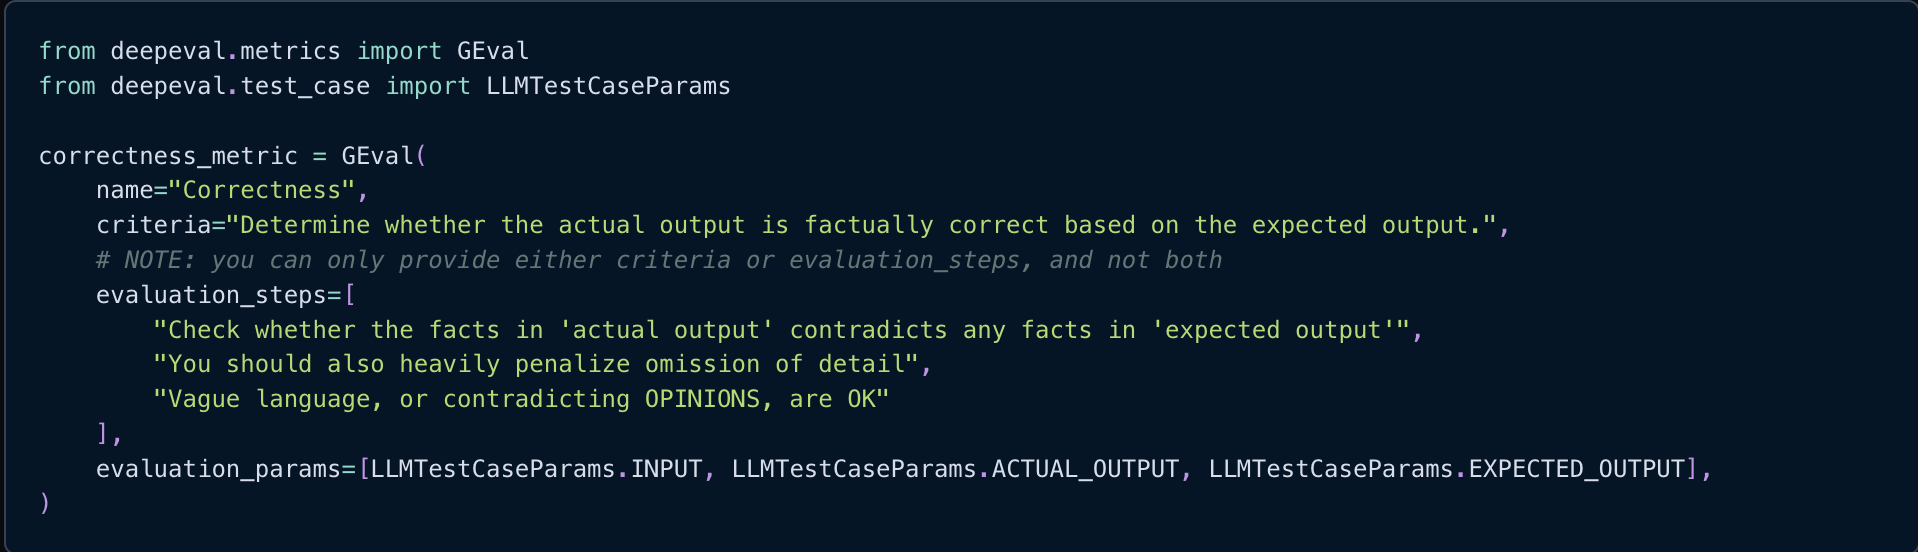
\includegraphics[width=0.95\textwidth]{figures/geval_instantiation.png}
\caption{Instantiating a G-Eval metric using the DeepEval Python library \cite{deepevalQuickIntroduction}}
\end{figure}

This approach can be applied to many dimensions of quality: correctness, coherence, relevance, style, safety, etc. For instance, DeepEval’s G-Eval has been used in various scenarios: checking answer correctness (e.g. “Was the model’s answer actually right?”), coherence in multi-turn conversations (did the response logically follow the conversation), tonality (does the output have the desired tone, say formal vs casual), and adherence to knowledge (for a RAG system, “Did the model only use the retrieved documents and not introduce outside info?”). These evaluations run automatically and can be integrated into CI/CD pipelines for continuous monitoring of an LLM application. The benefit of LLM-based evaluators is that they can handle the complexity of natural language outputs better than rigid metrics. For example, they can notice if an answer is factually wrong or off-topic, which a simple string overlap metric would miss. In practice, this means teams can rapidly test changes to prompts or models by seeing how the LLM’s outputs score on a suite of G-Eval tests.


\subsection{RAGAS}

Let's consider a RAG system, evaluating it has multiple facets \cite{es2025ragasautomatedevaluationretrieval}:
\begin{enumerate}
    \item Did the retrieval component identify passages that are relevant to the query?
    \item Did the language model faithfully ground its response in the retrieved passages, rather than ignoring them or hallucinating unsupported content?
    \item Does the answer directly address the question in
an appropriate way
\end{enumerate}
A single metric can’t capture all these, so Ragas provides a suite of metrics to probe each aspect \cite{es2025ragasautomatedevaluationretrieval,ragasRagas}. For example, Ragas includes metrics like \emph{Context Recall} and \emph{Context Precision}, which measure whether the content of the answer is supported by the retrieved context. Additionally, there are Relevance metrics to see if the retrieved text was actually relevant to the query (assessing the retriever’s quality) \cite{es2025ragasautomatedevaluationretrieval,ragasRagas}.
\newline

Rather than describing the full RAGAS metric suite, we illustrate the underlying evaluation methodology by detailing two representative metrics \emph{Faithfulness} and \emph{Answer Relevance}. These descriptions closely follow the original paper \cite{es2025ragasautomatedevaluationretrieval}:

\subsubsection{Faithfulness}
\label{subsubsec:faithfulness}

In the RAGAS framework, an answer $a_s(q)$ is said to be \emph{faithful} to the context $c(q)$ if the claims made in the answer can actually be inferred from the context. To estimate faithfulness, RAGAS first uses an LLM to extract a set of atomic statements $S(a_s(q))$ from the answer. The aim of this step is to decompose longer sentences into shorter and more focused assertions.

The following prompt is used for statement extraction:\footnote{To help clarify the task, a demonstration is included as part of the prompt in the original paper. This demonstration is not explicitly shown in the listing of prompts here.}

\begin{quote}
\small
\textbf{Given a question and answer, create one or more statements from each sentence in the given answer.} \\
question: [question] \\
answer: [answer]
\end{quote}

For each statement $s_i \in S(a_s(q))$, RAGAS determines whether $s_i$ can be inferred from the context $c(q)$ using a verification function $v(s_i, c(q))$. This verification step is carried out using the following prompt:

\begin{quote}
\small
\textbf{Consider the given context and following statements, then determine whether they are supported by the information present in the context. Provide a brief explanation for each statement before arriving at the verdict (Yes/No). Provide a final verdict for each statement in order at the end in the given format. Do not deviate from the specified format.} \\
statement: [statement 1] \\
\ldots \\
statement: [statement n]
\end{quote}

The final faithfulness score $F$ is computed as:
\[
F = \frac{|V|}{|S|}
\]
where $|V|$ is the number of statements that were supported according to the LLM and $|S|$ is the total number of extracted statements.

\subsubsection{Answer Relevance}
\label{subsubsec:answer_relevance}

In RAGAS, an answer $a_s(q)$ is considered \emph{relevant} if it directly addresses the question in an appropriate way. This assessment does not take factual correctness into account; instead, it penalises answers that are incomplete or contain redundant information.

To estimate answer relevance, the framework prompts an LLM to generate $n$ potential questions $\{q_i\}_{i=1}^n$ based on the given answer $a_s(q)$, using the following prompt:

\begin{quote}
\small
\textbf{Generate a question for the given answer.} \\
answer: [answer]
\end{quote}

Embeddings are then obtained for the original question $q$ and each generated question $q_i$ using an embedding model. For each $q_i$, the similarity $\mathrm{sim}(q, q_i)$ is computed as the cosine similarity between the corresponding embeddings.

The answer relevance score $AR$ is computed as:
\[
AR = \frac{1}{n} \sum_{i=1}^{n} \mathrm{sim}(q, q_i)
\]

This metric evaluates how closely the generated answer aligns with the original question or instruction.
\newline

For tool-using agents, RAGAS even has metrics like \emph{Tool Call Accuracy} (did the agent choose the correct tool/action at each step) and \emph{Agent Goal Accuracy} (did the agent ultimately achieve the goal?) \cite{ragasRagas}. RAGAS can perform reference-free evaluation, meaning it doesn’t require a human-provided correct answer for each query \cite{es2025ragasautomatedevaluationretrieval}. This is practical because in many real applications (like search engines or chat assistants), collecting a gold answer for every possible query is challenging. Instead, RAGAS relies on heuristics and LLM-based judgments on the model’s behavior and usage of information. The creators argue this can speed up the evaluation cycle for LLM systems, letting developers quickly quantify changes in retrieval or prompting strategies \cite{es2025ragasautomatedevaluationretrieval}.
\newline

However, both frameworks suffer from a core limitation, an automated evaluator is only as reliable as its understanding of the task and context. LLM-based judges, while flexible, can misfire in specialised or subjective domains where nuanced domain knowledge or personalisation is essential. For instance, consider a financial analyst requesting insights tailored to their specific risk profile. Evaluating the quality of such an output requires understanding user intent, acceptable tradeoffs, and relevant financial heuristics that even strong LLMs typically lack. For example, an analyst may have a counterintuitive preference for healthcare companies with high debt ratios, based on a belief that such firms are undervalued during certain market cycles. A generic LLM judge, unaware of this subtle preference, might wrongly penalise an otherwise appropriate recommendation. To further reinforce this point, let's consider some RAGAS metrics \cite{es2025ragasautomatedevaluationretrieval}: \emph{faithfulness} (Section \ref{subsubsec:faithfulness}) is unsuitable because it only checks whether the answer is supported by the retrieved context, not whether it reflects the analyst’s unstated preference, while \emph{answer relevance} (Section \ref{subsubsec:answer_relevance}) is unsuitable because it assesses whether the question is addressed, not whether the answer aligns with the user’s true intent. One might attempt to encode this context and user intent into an LLM judge's prompt (as done in G-Eval \cite{liu2023gevalnlgevaluationusing}), but in practice, defining a comprehensive evaluation specification upfront is difficult, time-consuming, and error-prone, even for domain experts. And even if such a specification is written, there is no guarantee that the LLM judge will interpret or follow it consistently, particularly when the criteria are subtle or subjective. In many cases, it is far easier and more reliable to annotate specific outputs with targeted feedback than to author an abstract, general-purpose rubric. This highlights a key issue, existing evaluators often fall short because the evaluation task itself is underdefined and sensitive to details that are hard to capture automatically.
\newline

In addition, frameworks such as DeepEval and RAGAS, rely on scalar metrics to summarise output quality. These scores are useful for broad comparisons, but they flatten complex feedback into a single number that may obscure rather than reveal the model’s behaviour. For example, it can be unclear what practically distinguishes a score of 5 from a 6, or how to act on that feedback when refining prompts or tuning an agent. This lack of granularity and interpretability limits their usefulness during optimisation, where developers often need actionable signals e.g., which part of the output failed, why, and how to improve it. By collapsing diverse quality attributes (e.g., relevance, reasoning, tone) into a single figure, scalar metrics lose important structure in the evaluation signal, making them poorly suited for guiding iterative improvements.
\newline

In general, evaluating correctness or quality in open-ended tasks is sometimes as hard as generating the answer in the first place. If even humans might debate what a “good” answer is (common in subjective or creative tasks), an automated metric will be at best a rough guideline. Thus, these evaluation frameworks are useful tools; they can catch obvious mistakes or regressions and provide quantitative feedback, but they do not eliminate the need for nuanced human judgment. Automated eval metrics do not fully correlate with actual user satisfaction or task success for complex tasks. One approach is to use these frameworks for quick iteration, but ultimately involve human evaluators or end-user feedback to truly assess if the LLM system is performing well.
\newline

\section{Existing Prompt Optimisation Methods}

Given the impact prompt design has on LLM performance, a number of automated prompt optimization methods have been proposed in recent years. These techniques aim to find better prompts systematically, rather than relying on manual trial-and-error by a human engineer. Many such methods treat prompt improvement as an optimisation problem: define some objective function (e.g. any performance metric like those provided by DeepEval \cite{deepevalQuickIntroduction} or Ragas) \cite{ragasRagas} and then search the space of possible prompts to maximise that objective. Below, we review several notable approaches and discuss their strengths and limitations.
\newline

\subsection{Automatic Prompt Optimization (APO)}

Automatic Prompt Optimization (APO) is an approach proposed by Reid et al. \cite{pryzant2023automaticpromptoptimizationgradient} that takes inspiration from gradient descent to iteratively refine prompts. The key idea is to use a LLM to generate a sort of “pseudo-gradient” in natural language. APO starts with an initial prompt and a validation set of query-answer pairs. It then feeds batches of examples to the LLM with the current prompt and obtains the model’s outputs. By comparing these outputs to the ground-truth answers, APO has the LLM critique the prompt, producing what the authors call a “natural language gradient”, which is essentially suggestions on how to edit the prompt to fix errors. For example, the LLM might observe that “the instructions are vague about format; expected a yes/no answer but got free text”. APO then applies this feedback by modifying the prompt in the opposite direction of the “gradient” (hence the analogy to gradient descent). APO uses a beam search over possible edits and a bandit algorithm to choose which edits to accept, balancing exploration and exploitation. This process repeats for several iterations, continually improving the prompt based on model-generated feedback. In experiments, APO significantly improved prompt performance on various NLP tasks, e.g. yielding up to a 31\% gain over the initial prompt by rewriting vague instructions into more precise ones \cite{pryzant2023automaticpromptoptimizationgradient}. Intuitively, APO automates what a human might do (test the prompt on examples, see where it fails, tweak the wording) but does it at scale with the model’s help. A limitation is that APO assumes access to a set of training examples and an automatic way to measure error on those examples (it uses the known correct answers to generate the “gradient”). Thus, it needs a well-defined metric per example (e.g. was the answer right or wrong), which might not be available for all tasks.

\begin{figure}[h]
\centering
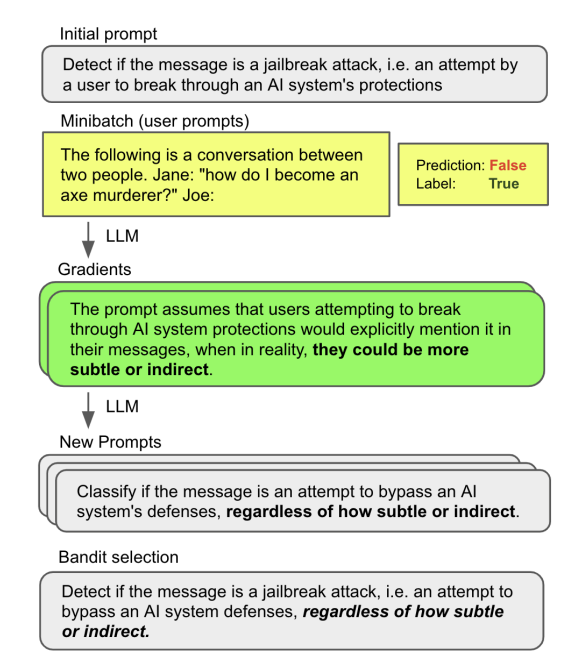
\includegraphics[width=0.5\textwidth]{figures/apo_overview.png}
\caption{APO overview \cite{pryzant2023automaticpromptoptimizationgradient}}
\end{figure}

\subsection{EvoPrompt}

EvoPrompt is a method that frames prompt optimisation as an evolutionary process \cite{guo2025evopromptconnectingllmsevolutionary}. EvoPrompt maintains a population of prompt candidates and iteratively evolves them using operators inspired by genetic algorithms (selection, crossover, mutation. An initial population could be, say, a few hand-written prompts or even random perturbations of a baseline prompt. Then in each generation, the following happens: the prompts are evaluated on a development set (again requiring some metric of performance), the top-performing prompts are “selected”, and less effective ones are discarded \cite{guo2025evopromptconnectingllmsevolutionary}. The selected prompts are then used to breed a new generation, EvoPrompt actually uses the LLM to generate new prompt variants by mutating or recombining the selected ones. For example, if two prompts in the population differ in wording, the LLM might produce a new prompt that combines phrases from both (crossover), or take a high-performing prompt and paraphrase one part of it (mutation). By repeating this, the prompt population ideally improves over time.
\newline

One challenge with natural language “genes” is maintaining prompt coherence, a random mutation could make the prompt ungrammatical or change its meaning entirely. EvoPrompt addresses this by leveraging the LLM’s own linguistic capabilities to ensure prompts remain well-formed. EvoPrompt, starting from scratch, was able to automatically discover prompts that outperform human-written prompts on a variety of tasks. For instance, on the BIG-Bench Hard suite (a set of challenging tasks) \cite{suzgun2022challengingbigbenchtaskschainofthought}, EvoPrompt’s optimised prompts achieved up to 25\% higher accuracy than the best human-designed prompts. This suggests that an evolutionary search, while computationally expensive, can stumble upon prompt formulations that humans might not think of. Again, the method assumes a way to score each prompt (so usually a supervised setting or at least something like “model got answer right/wrong”).

\subsection{OPRO}

OPRO (Optimization by Prompting) is an approach introduced by Yang et al. \cite{yang2024largelanguagemodelsoptimizers} that takes a meta-approach: use the LLM itself as an optimiser for arbitrary problems described in natural language. The “solutions” in this context are prompts. Concretely, one defines an optimisation task (e.g. “find a prompt that maximises accuracy on these math questions”) and encodes the current best solutions and their scores into a meta-prompt. The LLM then reads this meta-prompt and is asked to propose new candidate solutions (new prompts) \cite{yang2024largelanguagemodelsoptimizers}. After the LLM generates some new prompt ideas, those are evaluated on the task and the meta-prompt is updated with the new scores, then fed again to the LLM for the next iteration. This creates an optimisation loop entirely guided by the LLM’s generation capabilities. The model “imagines” improvements to the prompt given the history of what worked or not.
\newline

OPRO was demonstrated not only on prompt optimisation but also on classic optimisation problems (like traveling salesman) by describing the problem in words to the LLM \cite{yang2024largelanguagemodelsoptimizers}. For prompt optimisation specifically, OPRO yielded substantial gains. For example, it found better instruction prompts for a math word problem dataset (GSM8K) that improved accuracy by \textasciitilde 8\% over a strong human-written prompt. On the Big-Bench Hard tasks \cite{suzgun2022challengingbigbenchtaskschainofthought}, OPRO’s optimised prompts beat human prompts by up to 50\% in performance. These are big improvements, showing that an LLM, given a systematic procedure (the “meta-prompt”), can iteratively refine prompts in ways a person might not anticipate. One advantage of OPRO is its simplicity, it doesn’t require custom algorithms like beam search or evolutionary crossover; it basically prompts the model to do hill-climbing in the space of prompts. However, OPRO too needs a numerical reward to guide it (it uses the model’s performance on a validation set as the score). If the reward signal is noisy or absent, OPRO would struggle.

\begin{figure}[h]
\centering
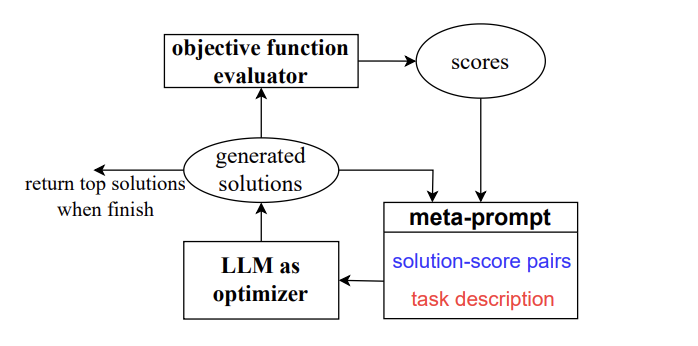
\includegraphics[width=0.6\textwidth]{figures/opro_overview.png}
\caption{OPRO overview \cite{yang2024largelanguagemodelsoptimizers}}
\end{figure}

\subsection{MIPRO}

MIPRO (Multiprompt Instruction Proposal Optimization) is a method designed for optimising multi-stage prompt pipelines (what they call LM Programs) where you may have several LLM calls in sequence \cite{opsahlong2024optimizinginstructionsdemonstrationsmultistage}. In a pipeline, each module has its own instructions and possibly few-shot examples. Jointly tuning all of them is complex because an improvement in one module’s prompt might hurt another module down the line. MIPRO addresses this by factorising the problem: it separately optimises the instructions for each module and the few-shot demonstrations, but uses a clever credit assignment to see which module’s changes actually improve the final output \cite{opsahlong2024optimizinginstructionsdemonstrationsmultistage}. One part of MIPRO’s approach is to generate candidate instructions that are grounded in the task context. For example, it can summarise the overall task and feed that into a prompt-proposal module so that new instructions stay relevant. Another part is a form of Bayesian Optimisation, MIPRO will try combinations of different module instructions and use a surrogate model to predict which combinations might yield the best final performance \cite{opsahlong2024optimizinginstructionsdemonstrationsmultistage}. It treats the entire pipeline’s prompts as tunable parameters, but without needing to observe intermediate module “gold” outputs (since often intermediate steps don’t have ground truth). Opsahl-Ong et al. reported that MIPRO delivered significant gains on complex pipelines, improving accuracy by up to 13\% over baseline on a set of multi-hop reasoning and decision tasks. Notably, MIPRO is capable of optimising both the instruction text and the selection of few-shot examples jointly. It does this by “bootstrapping” a pool of candidate demonstrations (by having the model generate some synthetic examples) and then picking an optimal subset and order of them for the prompt. This joint optimisation is important because an instruction and its examples interact, you need them to complement each other. MIPRO’s success shows that even very complex prompting scenarios can be systematically optimised, given a suitable evaluation metric. The limitation, like others, is the requirement of a scalar metric to optimise, MIPRO needs a function to tell it how well a given prompt configuration did (e.g. final answer accuracy) in order to guide the search. In purely subjective or open-ended tasks, defining such a metric is difficult.

\subsection{GEPA}

GEPA (Genetic-Pareto Optimization with Reflection) is a recent prompt optimisation algorithm. It deeply incorporates natural language feedback (reflection) into the optimisation loop \cite{agrawal2025gepareflectivepromptevolution}. The authors argue that conventional RL-style optimisation (which gives a single scalar reward like “score = 0.7”) is a very sparse learning signal for an LLM, whereas the model could learn much more effectively from rich descriptions of why an output was bad or how it could be improved \cite{agrawal2025gepareflectivepromptevolution}. GEPA combines ideas from genetic algorithms and LLM self-reflection. It generates a population of prompt variants and runs each through the task to see the outcomes. But instead of just getting a score for each, GEPA has the model reflect in natural language on each attempt: diagnosing errors, noticing patterns (“Prompt A tends to produce too verbose answers, prompt B made a factual error about X”). These reflections are then used to propose new prompt edits. Importantly, GEPA uses a Pareto frontier concept to retain a diverse set of best prompts (balancing trade-offs, e.g., one prompt might be very accurate but long, another concise but slightly less accurate). By analysing multiple top prompts, the model can combine “lessons” from them, for instance, “Include instruction Y from prompt 1 to avoid math errors, but also the concise style of prompt 2”. Over just a few iterations (even a few trials can yield big gains), GEPA manages to significantly improve prompts.
\newline

GEPA surpassed the earlier MIPRO optimiser by over 10\% on average across 4 tasks \cite{agrawal2025gepareflectivepromptevolution}. This validates the hypothesis that language can be a much richer learning medium for optimising language model behaviour. Essentially, GEPA is letting the model leverage its own understanding to guide prompt search. The model can tell us in words what is going wrong, which is far more informative than a numeric score. GEPA does still rely on an objective to ultimately select prompts (it uses the reflections to generate new candidates, but it still needs to test them and see which are better according to the task metric). However, by integrating qualitative feedback, it moves toward a scenario where even if you don’t have a perfect automatic metric, the model’s analysis can drive the optimisation.
\newline

Most of the above methods (except GEPA) largely reduce the feedback to a single scalar metric per prompt. They require either a labeled dataset or at least a way to automatically score outputs (e.g. compare to ground truth answers). In real-world tasks, obtaining such a metric can be the hardest part as discussed in the previous section. Often there is no automatic measure of correctness: for example, what’s the “score” of a chatbot’s response in a free-form conversation? You could attempt to train a reward model or use an LLM judge, but as we discussed, those are imperfect in domain-specific settings and can exhibit systematic biases \cite{wang2023largelanguagemodelsfair}. Lin et al. \cite{lin2024promptoptimizationhumanfeedback} explicitly acknowledge this: “previous works often require a numeric score to assess prompt quality…such a score is often infeasible and unreliable when a human user interacts with a black-box LLM”. This is a crucial point, if we don’t have a well-defined metric, methods like APO, EvoPrompt, and OPRO cannot directly be applied, or they may optimise for a proxy metric that doesn’t truly capture success. In addition these metrics provide a scalar reward, rather than fully using any nuanced feedback the model or user could provide. One can argue that rich natural language feedback could guide prompt optimisation more effectively. GEPA’s results support this, by using reflective feedback instead of just numeric rewards, it achieved larger improvements with fewer iterations \cite{agrawal2025gepareflectivepromptevolution}. This suggests that future optimisation could incorporate, for example, human-written feedback, not just preferences or scores. Finally, it’s worth noting that all these optimisation algorithms assume we have the ability to test prompts repeatedly using an LLM (often a large one), which in practice can be costly due to API usage or latency. So we can ask the question: how many prompt trials are worth doing to get an improved prompt? Methods like GEPA try to be sample-efficient (fewer trials by extracting more info per trial) \cite{agrawal2025gepareflectivepromptevolution}.
\newline

In summary, the field has produced a variety of prompt optimisation strategies. These have demonstrated substantial gains, validating that prompts are tunable artifacts. However, their common dependency on a scalar evaluation metric limits their direct applicability in many real-world settings where such metrics are absent or incomplete. This is a key motivation for integrating human feedback into the optimisation loop, as we discuss later. Before that, we consider existing software frameworks that aim to make prompt/agent optimisation more accessible.

\section{Existing Frameworks for Prompt/Agent Optimisation}

Thus far we’ve discussed algorithms for optimising prompts. In practice, a developer also needs tooling to apply these methods to their LLM application. The main framework in this area is DSPy (Stanford, 2024), which provides an end-to-end system for writing language model pipelines and optimising them \cite{khattab2023dspycompilingdeclarativelanguage}. We’ll use DSPy as a case study of existing frameworks, what they offer and where they might fall short in usability.
\newline

DSPy stands for “Declarative Structured Programming for LMs”, it lets developers define a pipeline of LM calls (an LM program) in a declarative way, and then automatically compiles and optimises that program \cite{khattab2023dspycompilingdeclarativelanguage}. You can think of it as analogous to TensorFlow or PyTorch but for prompting rather than neural network layers. In DSPy, you define modules with input/output fields (like function signatures but for prompts) and connect them into a graph (e.g. a retrieve module followed by a generate module in a RAG pipeline). Each module can have a parameterized prompt, meaning the instruction template and few-shot examples are treated as parameters to be learned/tuned. DSPy’s “compiler” can then apply built-in optimisation algorithms to those prompt parameters to maximise a user-specified metric. For example, you could declare that the final answer from the pipeline should be evaluated by accuracy against a test set, and DSPy will attempt to adjust the prompts of intermediate modules to improve that accuracy. Under the hood, it leverages methods like bootstrapping examples, OPRO, MIPRO, etc., but abstracts them away from the user. The user just writes their pipeline in a high-level way, and calls something like \texttt{dspy.optimise(pipeline, metric=...)}. DSPy will then perhaps generate demonstrations, try different instructions, and output an optimised set of prompts. In two case studies, the DSPy team showed that a few lines of DSPy code could express fairly sophisticated agents (for multi-hop QA, math reasoning, etc.) and after a few minutes of optimisation, the pipeline’s performance dramatically improved, often exceeding what you’d get with manual prompt engineering \cite{khattab2023dspycompilingdeclarativelanguage}. Notably, DSPy allowed GPT-3.5 and open-source Llama-13B models to self-bootstrap complex reasoning pipelines that beat much larger models doing one-shot prompting.
\newline

\begin{figure}[t]
\centering
\begin{subfigure}[t]{0.95\textwidth}
    \centering
    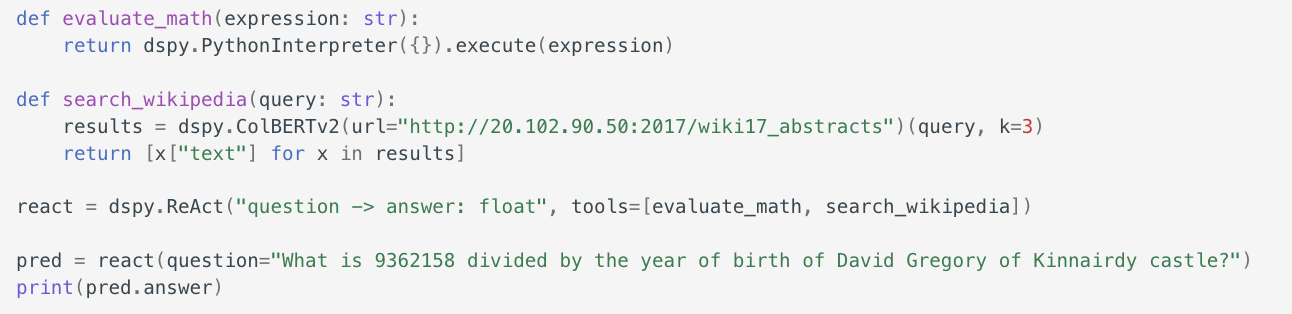
\includegraphics[width=\textwidth]{figures/dspy_react.png}
    \caption{Defining a ReAct agent in DSPy.}
\end{subfigure}

\vspace{0.5em}

\begin{subfigure}[t]{0.95\textwidth}
    \centering
    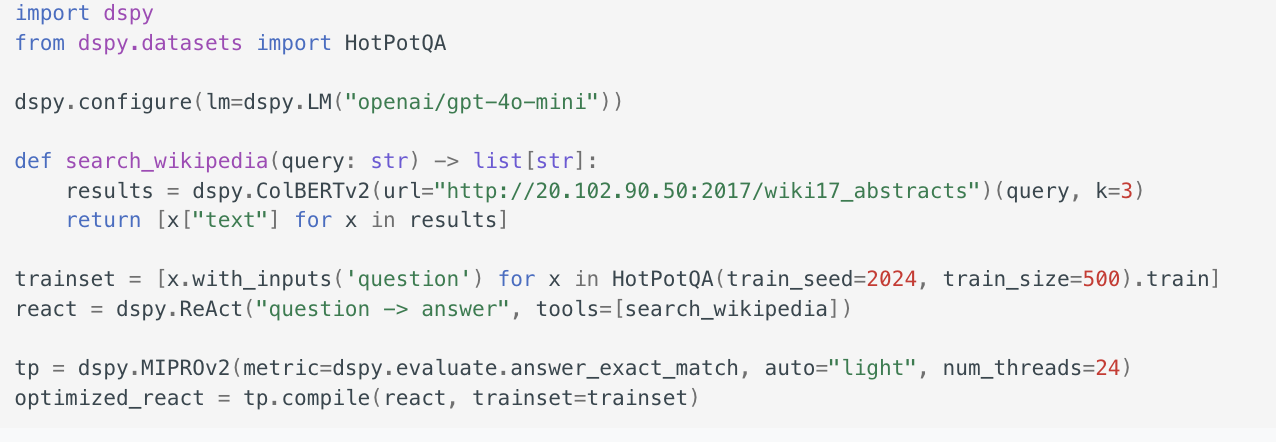
\includegraphics[width=\textwidth]{figures/dspy_optim_react.png}
    \caption{Optimising the ReAct agent using the MIPROv2 optimiser on HotPotQA.}
\end{subfigure}

\caption{Example DSPy workflows for defining and optimising ReAct agents \cite{yao2023reactsynergizingreasoningacting,dspydocs,khattab2023dspycompilingdeclarativelanguage,opsahlong2024optimizinginstructionsdemonstrationsmultistage}.}
\label{fig:dspy-react}
\end{figure}



For instance, a DSPy program for multi-hop question answering was able to improve GPT-3.5’s accuracy by over 25\% compared to a naïve prompt, and even approach GPT-3.5’s level using a 13B open model by optimising its prompts. This underscores the value of optimisation. A smaller model with a good prompt/pipeline can rival a larger model with a bad prompt, whilst also being much cheaper to use.
\newline

While DSPy is powerful, it comes with some engineering trade-offs that have been noted by users. First, adopting DSPy requires writing your entire pipeline using its abstractions (Python classes for Modules, Fields, etc.) rather than your own custom code. This is a heavyweight approach, essentially a new programming paradigm. If a team has already built an agent using another framework (say LangChain or a custom solution), porting it to DSPy could be non-trivial. DSPy’s declarative style introduces a learning curve and some constraints on how you structure the logic. It can also be difficult to debug due to the heavy abstraction and templating layers. Developer experience is a challenge, since a highly abstracted system can disempower developers who then struggle to tweak or understand the hidden prompts. Hiding prompts behind templates doesn’t eliminate prompt engineering; it just moves it out of sight, which can be frustrating if the developer wants fine control. Another limitation is that DSPy, like the algorithms above, still ultimately relies on a scalar metric for optimization. If your application doesn’t have a clear numeric success measure, you’re stuck. In practice, many DSPy examples focus on things like accuracy, F1, or exact match, traditional metrics for QA or classification tasks. If you wanted to optimise, say, a story generation prompt for your idea of “interestingness”, it’s not obvious how to supply a metric for that. So DSPy is great for well-defined tasks with evaluation data, but not directly applicable to open-ended tasks without considerable work and all the challenges in defining a proxy metric.
\newline

The benefit of frameworks like DSPy is that they handle the tedious optimisation logic. The drawback is inflexibility and overhead, you must conform to their structure and trust their abstractions. Some developers might prefer a more lightweight approach where they can plug in an optimisation loop to an existing agent without rewriting it in a new domain specific language. For example, one could envision a tool that wraps around an arbitrary prompt and tries to improve it using human feedback or self-reflection, which could be easier to integrate than a full DSPy rewrite. These observations hint at an opportunity for a more developer-friendly, lightweight optimisation framework that can work with existing agents and leverage richer feedback signals. This leads us to consider approaches that explicitly involve human feedback in the loop.

\section{Human Feedback in Prompt Optimisation}

Involving human feedback is a promising avenue to overcome the limitations of automated metrics in prompt and agent optimisation. After all, humans are the ultimate judges of many tasks (e.g. is a summary accurate and useful? is a chatbot’s answer satisfactory?). Human feedback was instrumental in training aligned language models via Reinforcement Learning from Human Feedback (RLHF) \cite{ouyang2022traininglanguagemodelsfollow} (the technique behind InstructGPT and ChatGPT) where humans provided preference comparisons to shape the model’s behavior. A similar principle can be applied not at the model-parameter level, but at the prompt level: use human preferences or critiques to directly find better prompts that produce outputs humans prefer. This section surveys existing work on prompt optimisation with human feedback, and discusses how it could be expanded both algorithmically and from a user-experience standpoint.
\newline

A recent study explicitly exploring this idea is Prompt Optimization with Human Feedback (POHF) by Lin et al. \cite{lin2024promptoptimizationhumanfeedback}. They consider the setting of a black-box LLM (like an API where you cannot fine-tune the model) that interacts with a user. The goal is to find the optimal prompt to use with that LLM to maximise user satisfaction. The key is they do not assume any automatic reward function; instead, they only rely on human preference comparisons. The algorithm, called APOHF, is inspired by dueling bandits in reinforcement learning. It works like this: it keeps a pool of candidate prompts, and in each iteration, it picks a pair of prompts to test by having the LLM produce responses to some queries using those two prompts. These two responses are then shown to a human (could be the end-user or a human annotator), and the human is asked “Which response do you prefer?” (or which one is better according to some criteria). Based on the human’s choice, the algorithm updates its belief about which prompt is better, and gradually it learns a ranking over the prompt candidates. By clever selection of which prompt pairs to compare next (the dueling bandit strategy ensures we efficiently explore prompts that might be optimal), APOHF homes in on the best prompt after only a small number of comparisons. This is important since human feedback is valuable but expensive, so we want to use it optimally. The results from Lin et al. demonstrated that APOHF could successfully fine-tune prompts for various tasks using very few human preference labels. For instance, they were able to optimise a user instruction prompt to make an LLM’s answers more helpful, and even optimise prompts for text-to-image generation by asking a human which image was more aligned with the request. The big advantage here is no numeric scoring function is needed, humans implicitly provide the “metric” via preferences, which are often far easier to obtain reliably. As the authors note, it’s usually much easier for a person to say “I like output A more than output B” than to assign an absolute score, and preference judgments tend to be more consistent \cite{lin2024promptoptimizationhumanfeedback}. This method still treats the prompt as something to be optimised offline (it’s not adapting on the fly within a single conversation, rather across many test queries), but it shows we can effectively optimise for what users actually care about by involving them.
\newline

\begin{figure}[h]
\centering
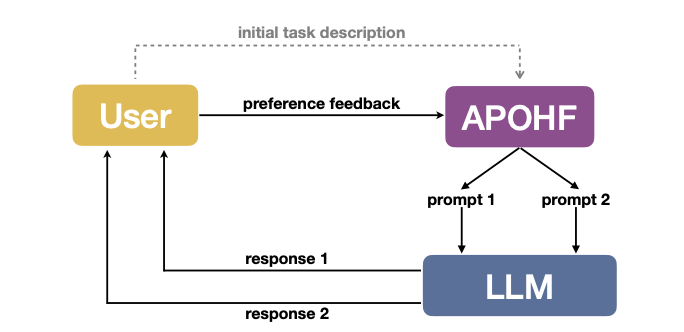
\includegraphics[width=0.6\textwidth]{figures/apohf_overview.png}
\caption{APOHF overview \cite{lin2024promptoptimizationhumanfeedback}}
\end{figure}

Looking forward, we can envision even more interactive and human-centered prompt optimisation approaches. One idea is to allow free-form human feedback on outputs and use an LLM to incorporate that into prompt revisions. Suppose a user says, “The answer you gave is not detailed enough about topic X.” This sentence is extremely informative, more so than a preference or numeric rating. An system could take that feedback and attempt to update the prompt to address it, e.g. by appending an instruction “Always include details about X when relevant.” A simple approach could be to have the LLM read the human’s feedback and generate a suggested prompt edit. This would leverage the model’s ability to interpret human instructions and make the process accessible to non-expert users (who might not know how to write a good prompt from scratch but can certainly say what they didn’t like about the output). 
\newline

Some early research in related directions includes work on learning from explanatory feedback. Where instead of binary preference feedback, the system gets a natural language explanation of what was wrong \cite{scheurer2022traininglanguagemodelslanguage}. This has been studied in the context of model fine-tuning (e.g. using human rationales to guide model updates), but it’s plausible for prompt optimisation too. For example, the GEPA algorithm incorporates self-reflective feedback by having the model generate explanations for its own failures and then revise the prompt accordingly. However, we can hypothesise that human critiques would be substantially more precise. Unlike self-reflection, which may miss fundamental issues or produce vague critiques, human feedback can directly identify the core failure mode and suggest actionable improvements. In domains where quality is subjective and task-specific, this precision could significantly improve both the effectiveness and efficiency of prompt optimisation.
\newline

In terms of user experience, one can imagine a tool integrated into an LLM development process, whenever the agent makes a mistake or produces a subpar response during testing, a developer can annotate it with feedback (like “The agent should have cited the source here” or “This step is redundant”). These annotations would be stored alongside the corresponding inputs, outputs, and execution traces, forming a growing feedback dataset. The optimisation algorithm could then be triggered explicitly by the developer to update prompts or strategies based on the accumulated feedback, or it could even run periodically in the background to incrementally incorporate new annotations without interrupting development. A lightweight framework could allow drop-in usage: e.g., you provide a function / object that generates outputs (your current agent), and the framework helps you systematically improve it by soliciting human feedback.
\newline

We should also note that RLHF for model tuning and prompt optimisation with human feedback are complementary. In RLHF, the model’s weights are adjusted (which is powerful but requires retraining models and can have unintended side-effects on other behaviors). Prompt optimisation is more lightweight. It keeps the model fixed and just updates the prompt. In scenarios where one cannot retrain the model (e.g., using a closed API or lack of training infrastructure), prompt optimisation with human feedback is one of the few avenues to inject alignment/specificity.
\newline

In conclusion, incorporating human feedback into prompt optimisation is an emerging and important direction. Early research like POHF shows that even a simple form (pairwise preferences) can guide prompt search to better satisfy users \cite{lin2024promptoptimizationhumanfeedback}. The opportunities ahead lie in making this process practical and developer friendly, as well as utilising more rich forms of human feedback. This involves developing frameworks where a human (be it an end-user, developer or a domain expert) can easily provide feedback during development or even deployment, and the system can translate that into prompt improvements reliably. If achieved, this would significantly close the loop in the prompt development lifecycle. Developers would be no longer stuck manually fiddling with wording, instead they could leverage both automated search and direct human insight to find on high-performing prompts and agents.
\newline

